\documentclass{uowmthesis}
\addbibresource{references.bib}

\setmainlanguage{greek}
\setotherlanguage{english}

\addbibresource{references.bib}

\begin{document}

% ========== keep your preferred covers ==========
% English
\begin{titlepage}

\selectlanguage{greek}

    \noindent
    \begin{minipage}[c]{0.49\textwidth}
        
\includegraphics[width=9cm,height=2cm,keepaspectratio]{logos/gr/uowm-logo-horizontal-gr.png}
    \end{minipage}%
    \hfill
    \begin{minipage}[c]{0.49\textwidth} 
        \raggedleft

        % uncomment if your lab has a logo
        % 
\includegraphics[width=4cm,height=1.8cm,keepaspectratio]{logos/isopt.eps}
    \end{minipage}

    \vspace{\fill}
    
    \vspace{3cm}
    
    \Large \centering \textbf{Τίτλος διπλωματικής}
    
    \vspace{\fill}
    
    \begin{center}
        \normalsize Διπλωματική εργασία \vspace{0.4em} \\
        \normalsize Ονοματεπώνυμο φοιτητή \vspace{0.4em} \\
    \end{center}

    
    
    \vspace{\fill}

    \begin{center}
        \normalsize Τμήμα Ηλεκτρολόγων Μηχανικών και Μηχανικών Υπολογιστών
        \vspace{0.4em} \\
        \normalsize Όνομα εργαστηρίου
        \vspace{0.4em}\\
        \normalsize Πολυτεχνική Σχολή 
    \end{center}

    \vspace{\fill}
    
    \begin{center}
        \normalsize Επιβλέπων:  \vspace{0.4em} \\
        \normalsize Ημερομηνία
    \end{center}


\end{titlepage}

% English
\begin{titlepage}
    \noindent
    \begin{minipage}[c]{0.49\textwidth}
        
\includegraphics[width=9cm,height=2cm,keepaspectratio]{logos/en/uowm-logo-horizontal-en.png}
    \end{minipage}%
    \hfill
    \begin{minipage}[c]{0.49\textwidth} 
        \raggedleft

        % uncomment to include lab logo
        % 
\includegraphics[width=4cm,height=1.8cm,keepaspectratio]{logos/isopt.eps}
    \end{minipage}

    \vspace{\fill}
    
    \vspace{3cm}
    
    \Large \centering \textbf{Thesis title}
    
    \vspace{\fill}
    
    \begin{center}
        \normalsize Diploma Thesis \vspace{0.4em} \\
        \normalsize Student name \vspace{0.4em} \\
    \end{center}

    
    
    \vspace{\fill}

    \begin{center}
        \normalsize Department of Electrical and Computer Engineering
        \vspace{0.4em} \\
        \normalsize Laboratory name
        \vspace{0.4em}\\
        \normalsize Faculty of Engineering 
    \end{center}

    \vspace{\fill}
    
    \begin{center}
        \normalsize Advisor: 
        \vspace{0.4em} \\
        \normalsize Date
    \end{center}


\end{titlepage}


% \begin{titlepage}
\selectlanguage{greek}

\begin{figure}[h!]
  \begin{center}
    \vspace{-1cm}
    
\includegraphics[width=3cm]{logos/uowm-logo.png}
    \label{fig:cover_uowm_logo}
  \end{center}
\end{figure}

\centering
\Large \tl{Πανεπιστήμιο Δυτικής Μακεδονίας}\\
\Large \tl{Πολυτεχνική Σχολή}\\
\large \tl{Τμήμα Ηλεκτρολόγων Μηχανικών και Μηχανικών Υπολογιστών}\\
\large \tl{Κατεύθυνση}

\vspace{\fill}

\LARGE \tl{Τίτλος διπλωματικής}

\vspace{\fill}

\Large \tl{Διπλωματική εργασία}\\
\Large \tl{του/της}\\
\Large \tl{Ονοματεπώνυμο}

\vspace{\fill}


\textbf{\tl{Επιβλέπων}:} \tl{}\\

\centering
\vspace{\fill}
\textbf{Ημερομηνία, ...}

\end{titlepage}
% \begin{titlepage}
\begin{figure}[h!]
  \begin{center}
    \vspace{-1cm}
    
\includegraphics[width=3cm]{logos/uowm-logo.png}
    \label{fig:cover_uowm_logo}
  \end{center}
\end{figure}

\centering
\Large \tl{University of Western Macedonia}\\
\Large \tl{Faculty of Engineering}\\
\large \tl{Department of Electrical and Computer Engineering}\\
\large \tl{Division name}

\vspace{\fill}

\LARGE \tl{Thesis title}

\vspace{\fill}

\Large \tl{Diploma Thesis}\\
\Large \tl{of}\\
\Large \tl{Student name}

\vspace{\fill}

\textbf{\tl{Supervisor}:} \tl{}\\

\centering
\vspace{\fill}
\textbf{Date, ...}

\end{titlepage}

% % English
\begin{titlepage}


\begin{figure}[h!]
  \begin{center}
  \vspace{-1cm}
    
\includegraphics[width=4.3cm]{logos/en/uowm-logo-vertical-en.png}
    \label{fig:cover_uowm_logo}
  \end{center}
\end{figure}

\vspace{\fill}

\Large \centering \textbf{Thesis title}

\vspace{\fill}

\begin{center}
    \normalsize Department of Electrical and Computer Engineering \\
    \normalsize Laboratory name \\
    \normalsize Faculty of Engineering
\end{center}

\vspace{\fill}

\begin{center}
    \normalsize Diploma thesis \\
    \normalsize of\\
    \normalsize Student name
\end{center}

\vspace{\fill}

\begin{center}
    \normalsize \textbf{Advisor:} \\
    \normalsize \textbf{Date}
\end{center}

\end{titlepage}

% % English
\begin{titlepage}

\begin{figure}[h!]
  \begin{center}
  \vspace{-1cm}
    
\includegraphics[width=4.3cm]{logos/gr/uowm-logo-vertical-gr.png}
    \label{fig:cover_uowm_logo}
  \end{center}
\end{figure}

\vspace{\fill}

\Large \centering \textbf{Τίτλος διπλωματικής}

\vspace{\fill}

\begin{center}
    \normalsize Τμήμα Ηλεκτρολόγων Μηχανικών και Μηχανικών Υπολογιστών \\
    \normalsize Όνομα εργαστηρίου \\
    \normalsize Πολυτεχνική Σχολή
\end{center}

\vspace{\fill}

\begin{center}
    \normalsize Διπλωματική εργασία \\
    \normalsize του/της \\
    \normalsize Ονοματεπώνυμο
\end{center}

\vspace{\fill}

\begin{center}
    \normalsize \textbf{Επιβλέπων:} \\
    \normalsize \textbf{Ημερομηνία}
\end{center}

\end{titlepage}


% ============ copyrights ============
\clearpage
\thispagestyle{empty}


{\normalsize \textbf{\en{Copyright} © \the\year{} Ονοματεπώνυμο φοιτητή, Επιβλέπων καθηγητής}}\\
Με επιφύλαξη παντός δικαιώματος. \en{All rights reserved}.\\
\newline
Απαγορεύεται η αντιγραφή, αποθήκευση και διανομή της παρούσας εργασίας, εξ
ολοκλήρου ή τμήματος αυτής, για εμπορικό σκοπό. Επιτρέπεται η ανατύπωση,
αποθήκευση και διανομή για σκοπό μη κερδοσκοπικό, εκπαιδευτικής ή ερευνητικής
φύσης, υπό την προϋπόθεση να αναφέρεται η πηγή προέλευσης και να διατηρείται το
παρόν μήνυμα. Ερωτήματα που αφορούν τη χρήση της εργασίας για κερδοσκοπικό
σκοπό πρέπει να απευθύνονται προς τον συγγραφέα.\\
\newline
Οι απόψεις και τα συμπεράσματα που περιέχονται σε αυτό το έγγραφο εκφράζουν
τον συγγραφέα και δεν πρέπει να ερμηνευτεί ότι αντιπροσωπεύουν τις επίσημες
θέσεις του Πανεπιστημίου Δυτικής Μακεδονίας.\\


Υπογραφή φοιτητή\\ 

............... .


\selectlanguage{english}
\clearpage
\thispagestyle{empty}

{\normalsize \textbf{Copyright © \the\year{} Student Name, Supervisor name}}\\
All rights reserved.\\
\newline
Copying, storing, and distributing this thesis, in whole or in part, for commercial purposes is prohibited. Reproduction, storage, and distribution for non-profit, educational, or research purposes are permitted, provided that the source is acknowledged and this message is preserved. Any inquiries regarding the use of this work for commercial purposes should be directed to the author.\\
\newline
The opinions and conclusions contained in this document express the views of the author and should not be interpreted as representing the official positions of the University of Western Macedonia.
% -------- include pdf declaration (optional) --------
% \includepdf[pages=-]{copyright_statement.pdf}


% =========== abstract ===========
\clearpage
\thispagestyle{empty}
\selectlanguage{greek}

\begin{abstract}

\par{Κείμενο περίληψης}

\par \textbf{Λέξεις κλειδιά}:
    
\end{abstract}
\selectlanguage{english}
\clearpage
\thispagestyle{empty}

\begin{abstract}
    \par {Abstract text}
    \par \textbf{Keywords}: 
\end{abstract}



% ======== acknowledgements ==========
\clearpage
\thispagestyle{plain}

\vspace*{\fill}
\begin{center}
  \vspace{-4cm} % adjust to remove title further up
  \textbf{Ευχαριστίες}
  
  \vspace{1.5em} % Adjust this for spacing between title and paragraph
  \parbox{0.75\textwidth}
  {%\centering
    Ευχαριστίες.
  }
\end{center}
\vspace*{\fill}
\clearpage
\thispagestyle{plain}

\vspace*{\fill}
\begin{center}
    \vspace{-4cm} % adjust to remove title further up
    \textbf{Acknowledgements}
  
    \vspace{1.5em} % Adjust this for spacing between title and paragraph
    \parbox{0.75\textwidth}
    {%\centering
        Your acknowledgements text is here.
    }
\end{center}
\vspace*{\fill}


\clearpage
\thispagestyle{empty}
\selectlanguage{greek}

\vspace*{\fill}
\begin{center}
    \Huge Τίτλος διπλωματικής \\
    \vspace{2cm}

    \normalsize Ονοματεπώνυμο φοιτητή \\
    \normalsize Email \\

    \vspace{1cm}
    \normalsize Ημερομηνία\\
\end{center}

\vspace*{\fill}



\clearpage
\thispagestyle{empty}
\selectlanguage{english}


\vspace*{\fill}
\begin{center}
    \Huge Thesis title \\

    \vspace{2cm}

    \normalsize Student name \\
    \normalsize \href{mailto:address}{Email} \\

    \vspace{1cm}
    \normalsize Date\\
\end{center}

\vspace*{\fill}

\selectlanguage{greek} % set main language again


% ======= include acronyms before contents =======
% \chapterheading{}{\acronymname}
% \newacronym{lp}{$LP$}{\en{Linear Programming}}
\newacronym{ai}{$AI$}{\en{Artificial Intelligence}}
\newacronym{cpu}{$CPU$}{\en{Central Processing Unit}}

\customtableofcontents
\customlistoftables
\customlistoffigures
\customlistofimages
\customlistofalgorithms


% ============ main body of your thesis ============

\chapter{Τίτλος κεφαλαίου}
\section{Τίτλος}


\begin{theorem}[Όνομα θεωρήματος]
Περιγραφή
\end{theorem}

\par Δοκιμαστικό κείμενο \gls{cpu}.


\begin{lemma}
Για κάθε $x\in\mathbb{R}$, ισχύει $x^2\geq 0$.
\end{lemma}
\section{Τίτλος}

\begin{image}
    \centering
    \begin{tikzpicture}
      \node[mybox] (start) {Έναρξη};
      \node[mybox, right=2cm of start] (process) {Διαδικασία};
      \node[mybox, below=1.5cm of process] (end) {Λήξη};
    
      \draw[myarrow] (start) -- (process);
      \draw[myarrow] (process) -- (end);
    \end{tikzpicture}
    \caption{Σύντομη περιγραφή}
    \label{img:test}
\end{image}


\chapter{Τίτλος κεφαλαίου}
\section{Τίτλος}
Παράδειγμα αναφοράς: \cite{BALABANOVJIANG2012}.

\begin{myalgorithm}{Όνομα αλγορίθμου - \en{Algorithm name}}{alg:conflict-res}
\begin{algorithmic}[1]
    \en{
        \Require Implication graph and a conflict at the current decision level
        \Ensure Learned clause and backjump level
        \Function{analyze\_conflict}{}
            \If{current\_decision\_level() == 0}
                \State \Return $-1$
            \EndIf
            \State $cl \gets$ find\_conflicting\_clause()
            \While{not stop\_criterion\_met($cl$)}
                \State $lit \gets$ choose\_literal($cl$)
                \State $var \gets$ variable\_of\_literal($lit$)
                \State $ante \gets$ antecedent($var$)
                \State $cl \gets$ resolve($cl$, $ante$, $var$)
            \EndWhile
            \State add\_clause\_to\_database($cl$)
            \State $back\_dl \gets$ clause\_asserting\_level($cl$)
            \State \Return $back\_dl$
        \EndFunction
    }
    \end{algorithmic}
\end{myalgorithm}

\section{Τίτλος}

\begin{figure}[h!]
    \centering
    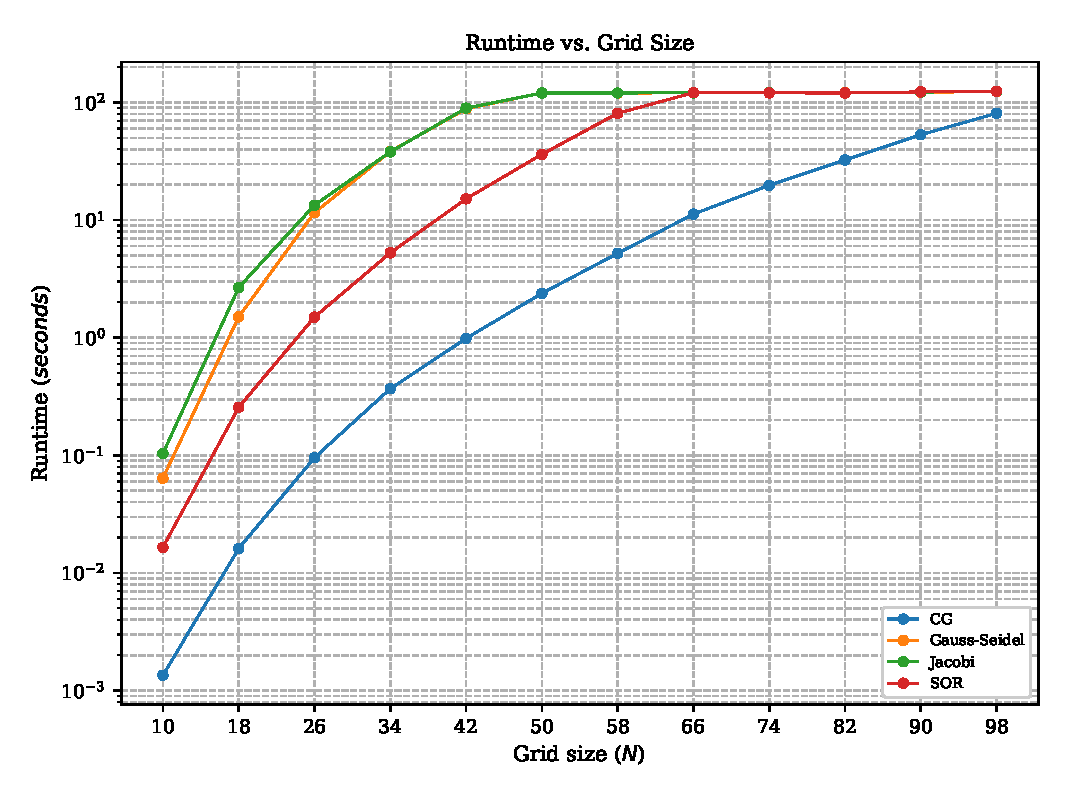
\includegraphics[width=0.80\linewidth]{doc/figures/runtime_gridsize.eps}
    \caption{Σύντομη περιγραφή}
    \label{fig:placeholder}
\end{figure}

\begin{image}
    \centering
    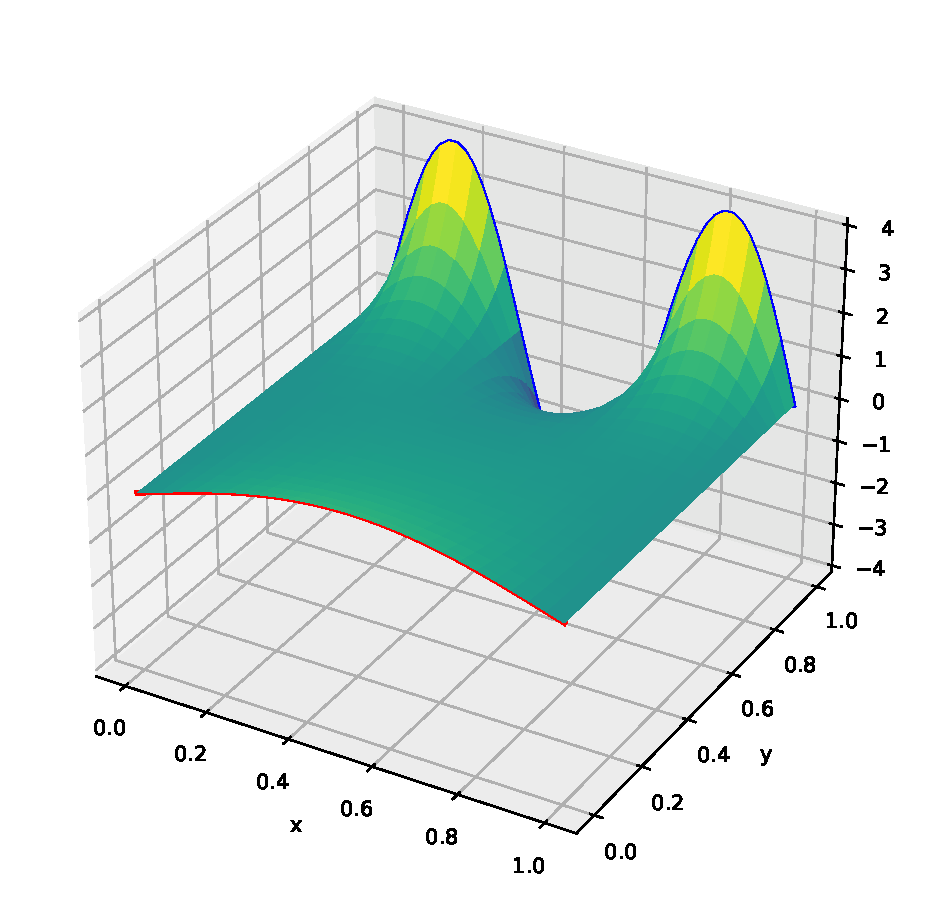
\includegraphics[width=0.70\textwidth]{doc/images/surface_plot.eps}
    \caption{Σύντομη περιγραφή}
    \label{img:example}
\end{image}


\begin{table}[h!]
    \centering
    \begin{tabular}{|c|c|c|c|c|}
    \hline
     N & \en{CG} & \en{Gauss-Seidel} & \en{Jacobi} & \en{SOR} \\
    \hline
    10 & 0.00104029 & 0.068981 & 0.107458 & 0.0152744 \\ \hline
    98 & 87.2408   & 2778.52  & 2843.33  & 1465.69    \\ 
    \hline
    \end{tabular}
    \caption{Σύντομη περιγραφή}
    \label{tab:computation-times}
\end{table}


% ============ appendices ============
\appendix
% ======= include acronyms in appendices =======
\appendixchapter{\acronymname}
\newacronym{lp}{$LP$}{\en{Linear Programming}}
\newacronym{ai}{$AI$}{\en{Artificial Intelligence}}
\newacronym{cpu}{$CPU$}{\en{Central Processing Unit}}

\appendixchapter{Κώδικας}
\begin{codeblock}{python}
def hello(name):
    print("Hello", name)
\end{codeblock}

\begin{codeblock}{c++}
#ifndef SOR_HPP
#define SOR_HPP

#include "utils/SolverLog.hpp"
#include "solvers/config.h"
template<typename Vector>
struct SOR
{   
    using Scalar       = typename Vector::Scalar;
    using SparseMatrix = Eigen::SparseMatrix<Scalar, Eigen::RowMajor>;

    double              tol       = DEFAULT_TOL;
    int                 max_iters = MAX_ITERS;
    double              omega;
    std::string         name      = "SOR";
    SolverLog<Vector>   log;
    Vector              final_solution;
    
    template<typename System>
    SOR (System system) : omega(system.omega_)
    {   
        log.system_dim     = system.A.rows();
        max_iters          = static_cast<int>(10 * std::sqrt(log.system_dim));
        log.max_iterations = max_iters;
        log.tolerance      = tol;
        log.solver_name    = name;
    }

    template<typename System>
    void solve(System& system)
    {   
        const auto& A        = system.A;
        const auto& b        = system.b;
              auto& u        = system.u;

        std::cout << "max_iters: " << max_iters << '\n';

        double sum1, sum2;
        
        double b_norm   = b.norm();
        double res      = (A * u - b).norm() / b_norm;

        if (res <= tol) 
        {   
            this->final_solution = u;
            log.final_solution   = this->final_solution;
            log.converged = 1;
            return;
        }

        Vector inv_diag = A.diagonal().cwiseInverse();

        for (int k = 0; k < max_iters; k++)
        {   
            for (int i = 0; i < A.rows(); ++i)
            {   
                double sum = 0;

                for (typename SparseMatrix::InnerIterator it(A, i); it; ++it)
                {
                    int j = it.col();

                    if (j != i)
                    {
                        sum += it.value() * u[j];
                    }
                }
                u[i] = (1 - omega) * u[i] + omega * (inv_diag[i] * (b[i] - sum));
            }
             
            res = (A * u - b).norm() / b.norm();

            log.num_of_iterations++;
            log.res_per_iteration.push_back(res);

            if (res <= tol) 
            {   
                this->final_solution = u;
                log.final_solution   = this->final_solution;
                log.converged = 1;
                return;
            }
        }
        this->final_solution = u;
        log.final_solution   = this->final_solution;
        return;
    }
};


#endif // SOR_HPP
\end{codeblock}

\begin{codeblock}{C++}
#ifndef CONJUGATE_GRADIENT_HPP
#define CONJUGATE_GRADIENT_HPP

#include "utils/SolverLog.hpp"
#include "solvers/config.h"
template< typename Vector>
struct ConjugateGradient
{
    double              tol       = DEFAULT_TOL;
    int                 max_iters = 1e6;
    std::string         name      = "CG";
    SolverLog<Vector>   log;
    Vector              final_solution;

    ConjugateGradient ()
    {
        log.tolerance      = tol;
        log.max_iterations = max_iters;
        log.solver_name    = name;
    }

    template<typename System>
    void solve(System& system)
    {   
        const auto&  A = system.A;
        const auto&  b = system.b;
        auto&        u = system.u;
        log.system_dim = A.rows();

        std::cout << "max_iters: " << max_iters << '\n';

        Vector r      = b - A * u; // initial residual
        double b_norm = b.norm();
        double r_norm = r.norm();

        if (r_norm / b_norm <= tol) 
        {   
            this->final_solution = u;
            log.final_solution   = this->final_solution;
            log.converged        = 1;
            return;
        }

        Vector d = r; // initial search direction
        Vector Ad(A.rows());

        for (int k = 0; k < max_iters; k++)
        {   
            // std::cout << "--------------------- iter. " << k+1 << " ---------------------\n";
            Ad.noalias() = A * d;

            double alpha      = ((r.transpose() * r) / (d.transpose() * Ad)).coeff(0); // step size
            double r_prev_dot = (r.transpose() * r).coeff(0); // to calculate beta

            u.noalias() += alpha * d;
            r.noalias() -= alpha * Ad;

            r_norm = r.norm();
            
            log.num_of_iterations++;
            log.res_per_iteration.push_back(r_norm / b_norm);

            if (r_norm / b_norm <= tol) 
            {   
                log.converged        = 1;
                this->final_solution = u;
                log.final_solution   = this->final_solution;
                return;
            }

            double beta = r.dot(r) / r_prev_dot;
            d           = r + beta * d; // update direction
        }
        this->final_solution = u;
        log.final_solution   = this->final_solution;
        return;
    }
};

#endif // CONJUGATE_GRADIENT_HPP
\end{codeblock}


% =========== bibliography ===========
\clearpage % remove if not needed
\chapterheading{}{\bibname}
\selectlanguage{english}
\printbibliography[heading=none]

\end{document}
